\documentclass[a4paper,10pt]{article}

% Encoding and typography
\usepackage[utf8]{inputenc}
\usepackage[T1]{fontenc}
\usepackage[scaled=0.95]{helvet}
\renewcommand{\familydefault}{\sfdefault}

% Page layout and visual elements
\usepackage[left=1.2cm, right=1.2cm, top=1.2cm, bottom=1.2cm]{geometry}
\usepackage{graphicx}
\usepackage{tikz}
\usepackage{enumitem}
\usepackage{titlesec}
\usepackage{xcolor}
\usepackage{hyperref}

% PDF metadata and link appearance
\hypersetup{
    colorlinks=true,
    linkcolor=blue,
    filecolor=magenta,
    urlcolor=blue,
    pdftitle={CV Marvyn Martinez},
}

% Global document style
\setlength{\parindent}{0pt}
\pagestyle{empty}
\titlespacing{\section}{0pt}{13pt}{4pt}

% Reusable CV structures
\newcommand{\cvsection}[1]{%
    \section*{#1}%
    \hrule
    \vspace{0.2cm}%
}

\newcommand{\educationentry}[4]{%
    \textbf{#1} | \textit{#2} \hfill \textit{#3} \\
    #4\par
}

\begin{document}

% Header
\begin{minipage}[m]{0.19\textwidth}
    \raggedright
    \begin{tikzpicture}
        \clip [rounded corners=0.3cm] (0,0) rectangle (2.5cm, 3.2cm);
        \node[anchor=south west, inner sep=0pt] at (0,-0.4) {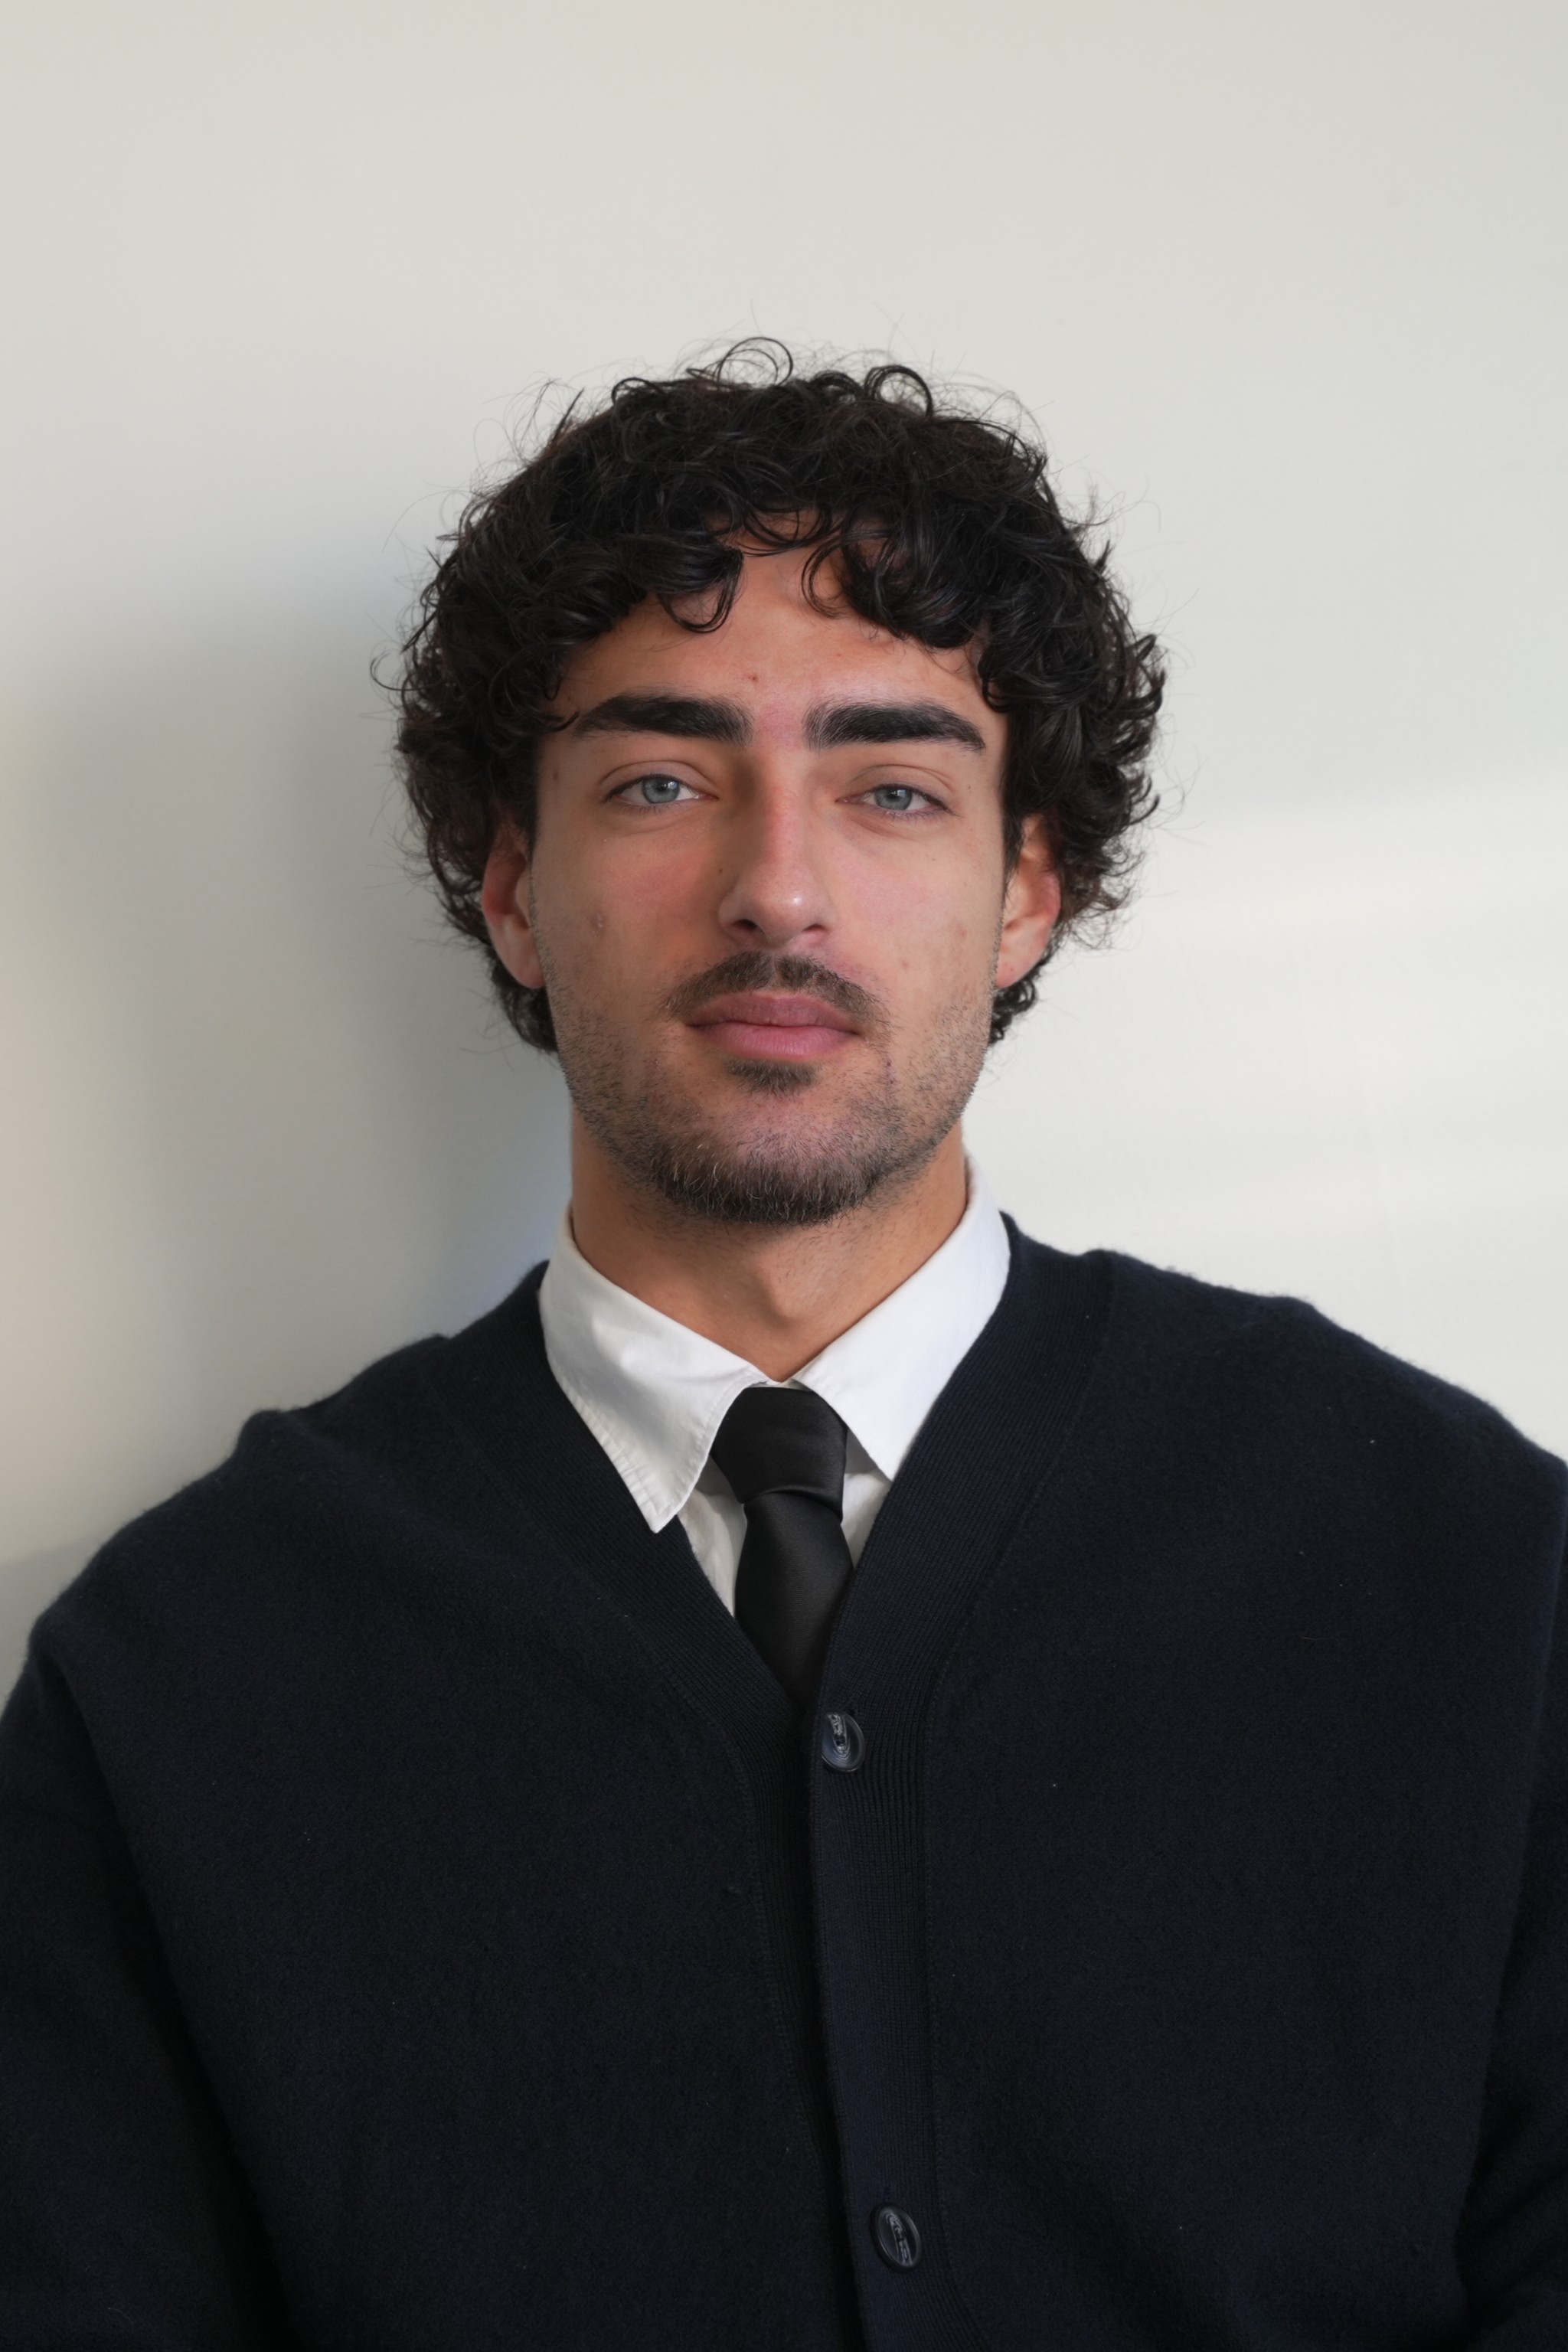
\includegraphics[width=2.5cm]{assets/photo.JPG}};
    \end{tikzpicture}
\end{minipage}
\begin{minipage}[m]{0.8\textwidth}
    \linespread{1.2}\selectfont
    {\huge \textbf{Marvyn Martinez}} \\
    {\large \color{gray} Data Engineer | Kafka - Spark - AWS} \\
    Paris, France | marvyn.martinez@icloud.com \\
    06.88.31.89.82 | \href{https://www.linkedin.com/in/marvyn-martinez/}{LinkedIn}
\end{minipage}

\linespread{1.45}\selectfont

% Skills
\cvsection{COMPÉTENCES}

\begin{itemize}[leftmargin=*, label={}, itemsep=2pt, parsep=0pt]
    \item \textbf{IA \& Analyse de données :} Python, Pandas, PyTorch, TensorFlow, Scikit-Learn
    \item \textbf{Data Engineering :} PySpark, Airflow, Kafka (Batch/Streaming), Snowflake, SQL 
    \item \textbf{Cloud \& Infrastructure :} AWS (S3, Lambda), Snowpark, Unix Shell
    \item \textbf{DevOps :} GitLab CI/CD, Confluence, Artifactory, JIRA, SonarQube
    \item \textbf{Observabilité \& BI :} Elasticsearch, Kibana, Tableau
    \item \textbf{Certifications :} TOEIC (805), Voltaire (797)
\end{itemize}

% Professional experience
\cvsection{EXPÉRIENCES PROFESSIONNELLES}

\textbf{Data Engineer} \hfill \textit{Sept. 2022 -- Août 2025} \\
\textbf{Bouygues Telecom} \hfill \textit{Meudon, France}

\begin{itemize}[leftmargin=*, itemsep=1pt, parsep=0pt, label={---}]
    \item Conception et pilotage de pipelines ETL/ELT multi-sources à forte volumétrie (JSON, Kafka -> Oracle/PostgreSQL) avec Python/Spark/Airflow - réduction du temps de traitement de 80\%.
    \item Garantie de la résilience des traitements : gestion des offsets Kafka (reprise sur incident), idempotence, tests unitaires et d'intégration automatisés, contrôles d'intégrité sur les flux de données.
    \item Développement de packages Python réutilisables (SQLAlchemy, Pandas, Spark, Snowpark, Kafka) pour standardiser les accès BDD et les contrôles qualité des traitements ETL/ELT.
    \item Mise en place du socle CI (GitLab CI/CD, Docker, Artifactory) avec les équipes DevOps pour automatiser les tests, le packaging et déploiement d’artefacts sur repository interne.
    \item Optimisation des performances SQL/Snowpark et Spark (partitionnement, plans d'exécution) - réduction des coûts compute et des temps d'exécution.
    \item Création de dashboards Tableau/Kibana pour data analysts, équipes métier (gestion d'incidents) et managers - +100 consultations/semaine.
    \item Rédaction et maintenance d'une documentation technique de 80+ pages sur Confluence ; animation d'ateliers techniques pour l'onboarding et le partage de connaissances.
    \item Travail en méthodologie Agile au sein d'une équipe de 6 personnes: daily, revues de code et sprints adaptés aux projets.
\end{itemize}

% Education
\cvsection{FORMATION}

\educationentry
    {ESIEE Paris}
    {Diplôme d'Ingénieur}
    {Août 2025}
    {Algorithmique, architecture logicielle et machine learning}

\vspace{0.3cm}

\educationentry
    {Heriot-Watt University Malaysia}
    {Master of Science}
    {Décembre 2024}
    {Stratégie d'entreprise et Leadership}

\vspace{0.3cm}

\educationentry
    {ESIEE Paris}
    {Classe Préparatoire (MPSI)}
    {Août 2022}
    {Mathématiques, Physique et Sciences de l'Ingénieur}

\end{document}
